\documentclass[10pt]{article}
\usepackage[letterpaper,margin=0.58in]{geometry}
\usepackage{booktabs}
\usepackage{tabularx}
\usepackage{graphicx}
\usepackage[font=small,skip=2pt]{caption}
\usepackage{xcolor}
\usepackage{microtype}
\usepackage[colorlinks=true,urlcolor=blue!60!black,linkcolor=black]{hyperref}
\usepackage{enumitem}
\setlist{nosep,leftmargin=*}
\setlength{\parindent}{0pt}
\setlength{\parskip}{3pt}
\usepackage{titlesec}
\titlespacing*{\section}{0pt}{5pt}{2pt}
\titleformat*{\section}{\normalsize\bfseries}
\newcolumntype{Y}{>{\raggedright\arraybackslash}X}

\title{\vspace{-1.8em}ITCS 8169 Assignment 2: Self-Supervised Visual Representation Learning}
\author{Jiaxiang Zhang}
\date{}

\begin{document}
\maketitle
\vspace{-2.9em}

\textbf{Code, trained models and instructions:} \url{https://github.com/JiaxiangCxx/ITCS8169_Assignment2}

\section*{1. Best result}
My best system reaches \textbf{88.25\% test accuracy (353 of 400 images)}. It averages the predictions
of three ResNet-18 networks. Each one started from random weights, first learned image features from
the training images \emph{without using their labels} (SimCLR), and was then fine-tuned with the labels.
No pretrained weights and no outside images were used.

To choose the system fairly, I held out 480 of the 2,400 training images as a validation set (30 per
class) and made every decision on it. The test set was only used to report results. Averaging three
networks gave 90.0\% validation accuracy, compared with about 89.5\% for a single network, so the
final system uses the average. Also checking a horizontally flipped copy of each test image did not
help on validation, so it is not used.

\section*{2. Supervised baseline}
The baseline is a ResNet-18 trained from random weights using only the labels: 224$\times$224 images,
200 epochs, AdamW (learning rate 0.001, weight decay 0.05), label smoothing 0.1, batch size 128, and
simple augmentation (random crops, flips and small brightness changes). It reaches
\textbf{83.4\% validation and 81.3\% test accuracy} (average of 3 runs). The main problem is
overfitting: it classifies 100\% of its training images correctly but only 83\% of the validation
images. With much stronger augmentation (RandAugment and MixUp/CutMix) it improves to 87.3\% / 84.6\%.

\section*{3. How the self-supervised learning works}
\textbf{Idea.} I used SimCLR. Each image is randomly changed twice (cropped, flipped, made brighter or
darker, blurred), which gives two ``views'' of the same picture. The network is trained so that the two
views of the same image get similar feature vectors, while views of different images get different
ones. A batch has 256 images, so each view must find its partner among 511 candidates. The only
way to do this is to recognize what stays the same under the changes, such as the shape and layout of
the scene, which is also what matters for classifying it. No labels are used in this stage.

\textbf{From features to a classifier.} After 500 epochs of this pretraining, I add a classification
layer and train the whole network on the labels with exactly the baseline settings. The only
difference from the baseline is therefore the starting point.

\textbf{What I adapted for this dataset.}
\begin{itemize}
\item \emph{Brightness and contrast changes are essential.} 15 of the 16 classes are grayscale photos.
Without these changes, the network can match two views just by their overall brightness and learns
little: the quality of its features drops from 81\% to 69\% (measured with a k-nearest-neighbor
classifier, which labels a validation image by its most similar training images).
\item \emph{Smaller crops help.} Allowing crops as small as 8\% of the image, instead of 20\%, forces the
network to connect a small part of a scene with the whole scene. A linear classifier on the frozen
features then improves from 81.3\% to 84.4\%.
\item \emph{Speed.} Changing images one at a time on the CPU took about 4 hours per pretraining run.
Doing it on the GPU for the whole batch takes 20 minutes, which made many experiments possible.
\item \emph{More unlabeled images.} For the final system, pretraining used all 2,400 training images
(still without labels).
\end{itemize}
I also tried two alternatives: \textbf{RotNet}, a simpler task where the network guesses how much an
image was rotated, and \textbf{joint training}, where the classification loss and the SimCLR loss are
trained at the same time instead of one after the other.

\section*{4. Results and analysis}
\begin{table}[t]
\centering
\small
\begin{tabularx}{\linewidth}{@{}Ycccc@{}}
\toprule
Method (all ResNet-18) & Runs & Validation (\%) & Test (\%) & Overfitting gap \\
\midrule
Supervised only (baseline) & 3 & 83.4\,$\pm$\,0.3 & 81.3\,$\pm$\,0.9 & 16.4 \\
Supervised only, strong augmentation & 3 & 87.3\,$\pm$\,0.4 & 84.6\,$\pm$\,1.4 & 12.7 \\
SimCLR, then train only a linear layer (network frozen) & 1 & 81.3 & 77.0 & -- \\
RotNet, then fine-tune & 1 & 85.0 & 80.3 & 14.2 \\
SimCLR, then fine-tune & 3 & 87.8\,$\pm$\,0.5 & 82.8\,$\pm$\,0.4 & 12.2 \\
Classification + SimCLR at once (brackets: SimCLR loss off) & 1 & 85.8 (86.3) & 81.5 (81.0) & 14.2 \\
SimCLR, then fine-tune with strong augmentation & 3 & 88.2\,$\pm$\,0.8 & 87.7\,$\pm$\,0.9 & 11.8 \\
\quad + smaller crops, pretraining on all 2,400 images & 3 & 89.5\,$\pm$\,0.1 & 86.6\,$\pm$\,1.1 & 10.5 \\
\textbf{Best: average of the 3 runs above} & -- & \textbf{90.0} & \textbf{88.25} & -- \\
\bottomrule
\end{tabularx}
\caption{Main results. $\pm$ is the standard deviation over runs. Overfitting gap = accuracy on the
training images minus validation accuracy (smaller is better).}
\end{table}
\begin{figure}[t]
\centering
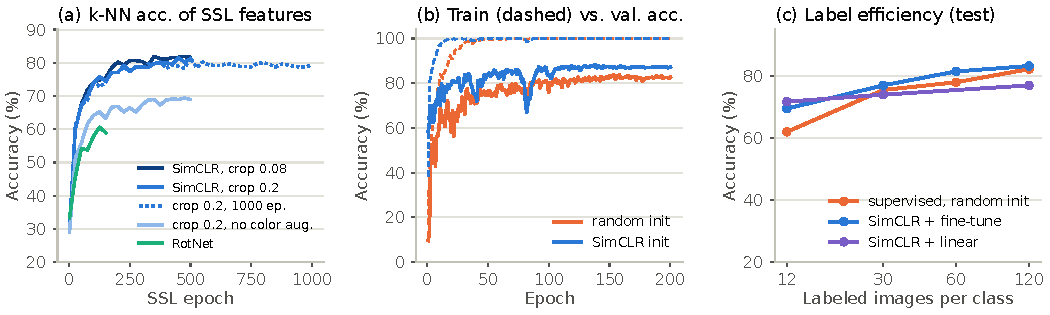
\includegraphics[width=\linewidth]{figures/analysis.pdf}
\caption{(a) Quality of the features during pretraining (k-nearest-neighbor accuracy on validation).
(b) Training accuracy (dashed) keeps rising to 100\% while validation accuracy (solid) stops; SimCLR
narrows the gap. (c) Test accuracy when only part of the labels is used.}
\label{fig:analysis}
\end{figure}

\textbf{SSL helps, mainly by reducing overfitting.} With the same training settings, starting from
SimCLR instead of random weights improves validation accuracy by 4.4 points and test accuracy by 1.6,
and shrinks the overfitting gap from 16 to 12 points (Fig.~\ref{fig:analysis}b).

\textbf{It helps most when labels are few.} With only 12 labeled images per class
(Fig.~\ref{fig:analysis}c), the baseline gets 62.0\%, SimCLR plus fine-tuning gets 69.5\%, and
simply training a linear layer on the frozen SimCLR features gets 71.8\%, because a frozen network
cannot overfit so few labels.

\textbf{SSL and strong augmentation work together.} Even when both sides use strong augmentation,
starting from SimCLR adds 3.1 test points (84.6\% to 87.7\%).

\textbf{A simpler task is worse, and longer training is not better.} RotNet's features are best
after 50 epochs and then get worse: the rotation can be guessed from easy clues such as where the
sky is, so the network stops learning anything useful about scenes. SimCLR stops improving after
about 500 epochs. By then it can tell the 1,920 training images apart 99.5\% of the time, so there
is little left to learn, and 1,000 epochs gave slightly worse features (79.4\% vs.\ 81.3\%). What
mattered most was the choice of image changes, not the training length.

\textbf{Training both goals at the same time did not help.} Joint training was no better than the
same setup without the SimCLR loss (85.8\% vs.\ 86.3\% validation), and keeping the SimCLR loss
during fine-tuning made it worse (86.9\% vs.\ 88.3\%). With so little data, the two goals seem to
compete; doing them one after the other works better.

\textbf{Bigger network.} Trained on labels only, ResNet-50 is worse than ResNet-18 (79.6\% vs.\
83.8\% validation) because it overfits more. With SimCLR pretraining it catches up (87.5\% vs.\
88.1\% validation) and does better on test (85.0\% vs.\ 83.3\%), so SSL helped the bigger network
more (one run each).

\section*{5. Limitations and conclusion}
\textbf{Limitations.} The evaluation sets are small: with 400 test images, one run's accuracy is
uncertain by about $\pm$1.7 points, so differences under about 2 points (for example between the last
three SimCLR rows of the table) are not reliable, and validation and test sometimes rank them
differently. Many side experiments were run only once. GPU memory limited the batch size, and I did
not try other methods such as MoCo, DINO or MAE. The final system runs three networks, so it is three
times slower at prediction. Finally, its validation accuracy is slightly optimistic because its
pretraining saw the validation images (without their labels).

\textbf{Conclusion.} Even with only 2,400 images, a network can learn useful features without labels.
Starting from those features makes the supervised training overfit less, and the benefit grows when
labels are scarce. The way the images are changed during pretraining, which encodes what we know about
the data, mattered more than which self-supervised method was used or how long it was trained.

\end{document}
